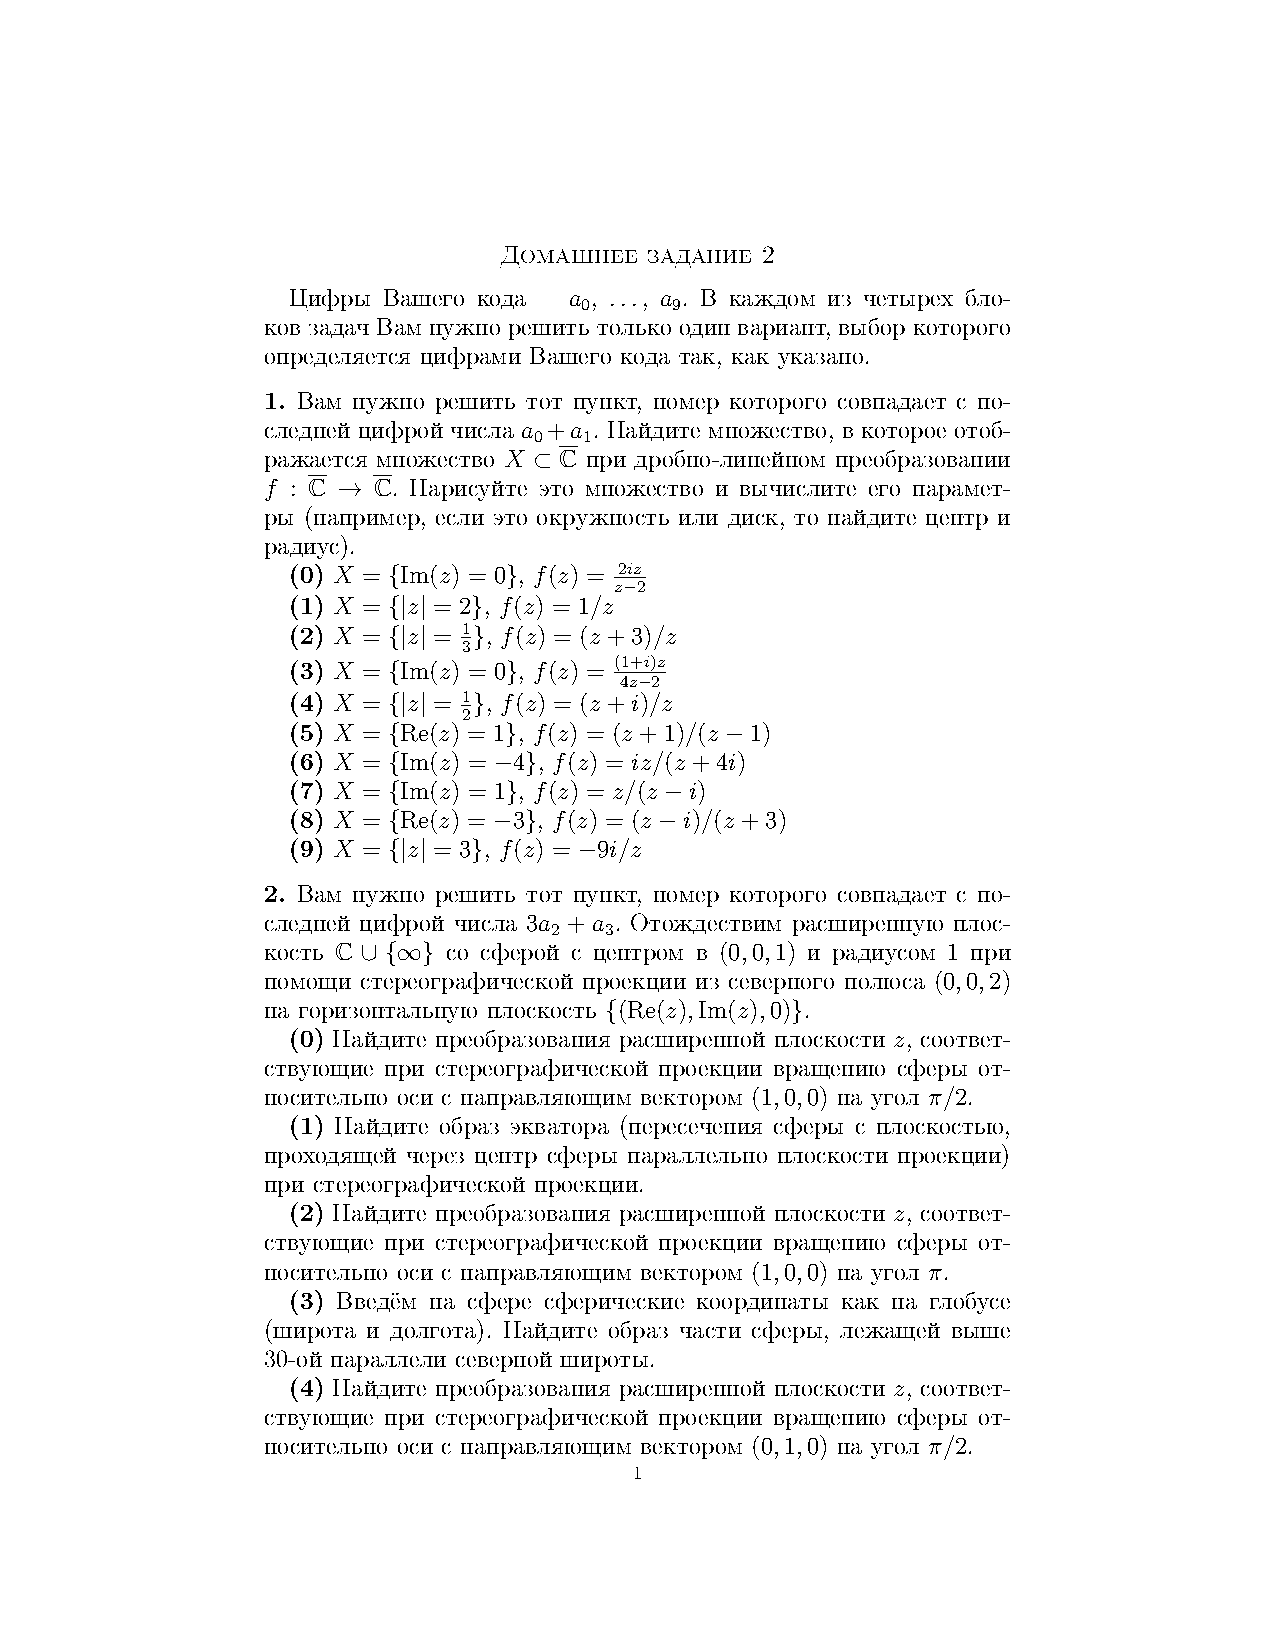
\includepdf[scale=1,pages=1-4]{Tasks/hw2}
\newpage
\section*{Решения}
\subsection*{Задача 1}
	Необходимо решить задачу $a_0 + a_1 = 1 + 7 = 8 \mod 10$
	\begin{gather*}
		X = \{\operatorname{Re}(z) = -3\},\ f(z) = \frac{z - i}{z + 3}\\
		\frac{(x + iy) - i}{(x + iy) + 3} = 1 - \frac{3 + i}{(x + iy) + 3}\\
		X:\ 1 - \frac{3 + i}{(x + iy) + 3} = 1 - \frac{3 + i}{(-3 + iy) + 3} = 1 - \frac{3 + i}{iy}
	\end{gather*}
	То есть мы получим прямую с выколотой точкой $z_0 = 1$
	\begin{figure}[!h]
		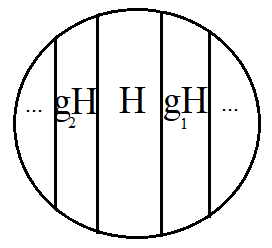
\includegraphics[width=0.5\linewidth]{Pic1}
	\end{figure}
\vskip 0.4in

\subsection*{Задача 2}
	Необходимо решить задачу $3a_2 + a_3 = 3 \cdot 8 + 9 = 3 \mod 10$\\
	Заметим, что часть сферы, лежащая выше 30-ой параллели является шапочкой данной сферы, точнее ее частью, лежащей выше $z = 1 + \sin(30) = 1.5$, тогда мы можем посмотреть, куда отображается эта параллель, а она отображается в окружность, точки которой имеют модуль $x = 2 \sqrt{3}$, то есть образ части сферы будет лежать вне этой окружности и задаваться формулой $z \overline{z} > (2\sqrt{3})^2 = 12$
\vskip 0.4in

\subsection*{Задача 3}
	Необходимо решить задачу $a_4 + 2a_5 = 7 + 2 \cdot 6 = 9 \mod 10$
	\begin{gather*}
		X = \{\operatorname{Re}(z) < 0,\ \operatorname{Im}(z) > 0\},\ f(z) = z^3 - i
	\end{gather*}
	Замеьтим, что при преобразовании $z \to z^3 - i$ модуль $z$ возводится в куб, аргумент умножается на 3, а затем результат сдвигается на $i$. Заметим, что аргументы элементов множества $X$ лежат в интервале $\left(\frac{\pi}{2}, \pi\right)$, а следовательно, после умножения на 3, аргументы будут лежать в $\left(\frac{3\pi}{2}, 3\pi\right)$. А следовательно в итоге будет множество $A = \mathbb{C} \backslash \{z \in \mathbb{C}:\ \operatorname{Re}(z) < 0,\ \operatorname{Im}(z) < -1\}$
\vskip 0.4in

\subsection*{Задача 4}
	Необходимо решить задачу $2a_6 + 3a_7 = 2 \cdot 9 + 3 \cdot 3 = 7 \mod 10$
	\begin{gather*}
		|z - i| - |z - 1| \leqslant 1\\
		|x + i(y - 1)| - |(x - 1) + iy| \leqslant 1\\
		\sqrt{x^2 + (y - 1)^2} + \sqrt{(x - 1)^2 + y^2} \leqslant 1\\
		x^2 + (y-1)^2 \leqslant 1 + (x-1)^2 + y^2 + 2\sqrt{(x-1)^2 + y^2}\\
		2x - 2y - 1 \leqslant 2\sqrt{(x-1)^2 + y^2}\\
		(2x - 2y - 1)^2 \leqslant 4(x^2 - 2x + 1 + y^2)\\
		(2x - 2y - 1)(2x - 2y - 1) = 4x^2 + 4y^2 - 8xy - 4x + 4y + 1 \leqslant 4x^2 - 8x + 4y^2 + 4\\
		-8xy + 4x + 4y \leqslant 3\\
		y(4 - 8x) \leqslant 3 - 4x
	\end{gather*}
	Тогда при $4 - 8x > 0:\ x < \frac{1}{2},\ y \leqslant \frac{3 - 4x}{4 - 8x}$ и при $4 - 8x < 0:\ x > \frac{1}{2},\ y \geqslant \frac{3 - 4x}{4 - 8x}$
	\begin{figure}[!h]
		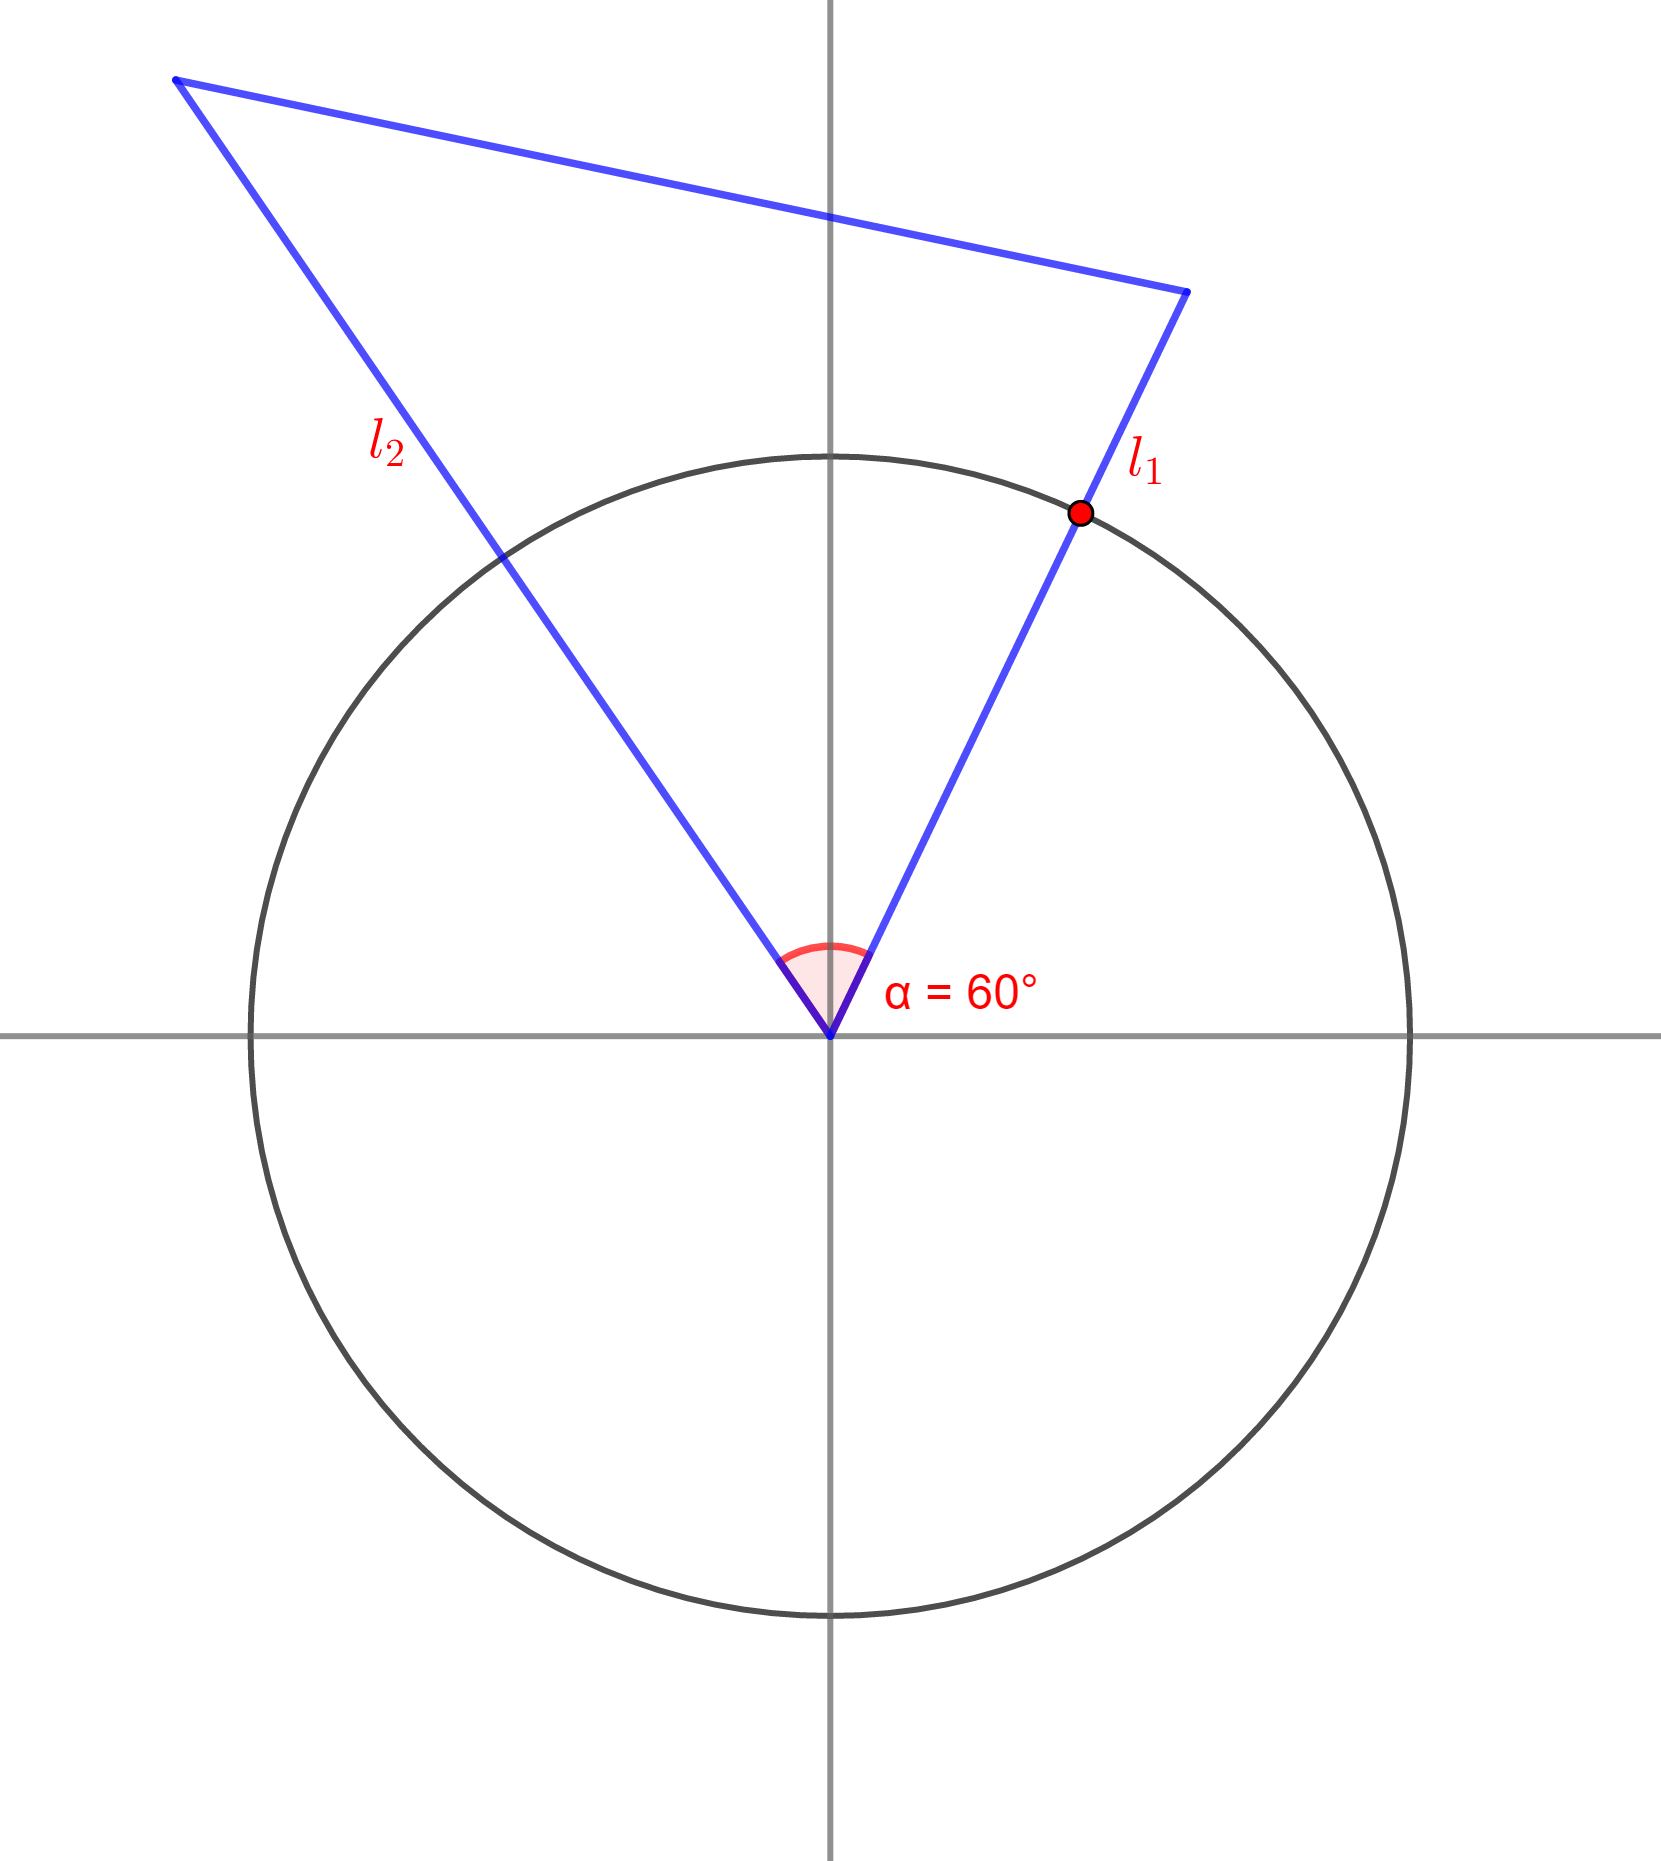
\includegraphics[width=0.5\linewidth]{Pic2}
	\end{figure}
\vskip 0.4in

\begin{comment}
\subsection*{Задача 5}
	Необходимо решить задачу $3a_0 + 4a_8 = 3 \cdot 1 + 4 \cdot 8 = 5 \mod 10$
	
\vskip 0.4in
\end{comment}
